\documentclass{article} % For LaTeX2e
\usepackage{nips14submit_e,times}
\usepackage{hyperref}
\usepackage{url}
\usepackage{amsmath,amsfonts,amsthm}
\usepackage{qtree}
\usepackage{natbib}
\usepackage{graphicx}
%\documentstyle[nips14submit_09,times,art10]{article} % For LaTeX 2.09


\usepackage{bm}
\def\B#1{\bm{#1}}
%\def\B#1{\mathbf{#1}}
\def\trans{\mathsf{T}}

%%%%%%%%%%%%%%%%%%%%%%%%%%%%%%%%%%%%%%%%%%%%%%%%%%%%%%%%%%%%%%%%%%%%%%%%%%%%%%%

\author{
Elvis DOHMATOB
\\
Parietal team, Inria Saclay Ile-de-France\\
Saclay, France\\
\textit{email}: firstname.lastname@inria.fr}

\title{Primal-dual algorithm for computing Nash equilibria in
% two-person zero-sum
sequential games with imcomplete information
% with imcomplete information and perfect recall
}


% The \author macro works with any number of authors. There are two commands
% used to separate the names and addresses of multiple authors: \And and \AND.
%
% Using \And between authors leaves it to \LaTeX{} to determine where to break
% the lines. Using \AND forces a linebreak at that point. So, if \LaTeX{}
% puts 3 of 4 authors names on the first line, and the last on the second
% line, try using \AND instead of \And before the third author name.

\newcommand{\fix}{\marginpar{FIX}}
\newcommand{\new}{\marginpar{NEW}}
\DeclareMathOperator{\prox}{prox}
\DeclareMathOperator{\im}{im}

\newtheorem{remark}{Remark}

\def \lb {{\langle}} \def \rb {{\rangle}}
\newcommand{\fro}[1]{\|#1\|_2}
\newcommand{\theHalgorithm}{\arabic{algorithm}}

\newcommand{\argmin}{\mathop{\mathrm{argmin}}}

\usepackage{hyperref}

\usepackage[ruled,vlined]{algorithm2e}
\usepackage{framed}
\newtheorem{theorem}{Theorem} \newtheorem{lemma}[theorem]{Lemma}
\newtheorem{proposition}[theorem]{Proposition}
\newtheorem{corollary}[theorem]{Corollary}
\newtheorem{definition}[theorem]{Definition}

%\nipsfinalcopy % Uncomment for camera-ready version
%%%%%%%%%%%%%%%%%%%%%%%%%%%%%%%%%%%%%%%%%%%%%%%%%%%%%%%%%%%%%%%%%%%%%%%%%%%%%%%

\begin{document}


\maketitle

\begin{abstract}
We present a simple primal-dual algorithm with a low cost per iteration, for computing Nash $\epsilon$-equilibria for two-person zero-sum sequential games with imcomplete information and perfect-recall like Texas Hold'em Poker, which converges after $\mathcal{O}(1/\epsilon)$ basic iterations (i.e iterations only involving basic operations like matvec, clipping, etc., and no calls to external first-order oracles, etc.). %% Our algorithm is applicable to a broad class of two-person zero-sum games including simultaneous games and sequential games with imcomplete information and perfect recall. The applicability to the latter kind of games is thanks to the sequen e-form representation von Stengel's \cite{von1996efficient}
Our algorithm derives from the general primal-dual algorithm developed
% by Chambolle and Pock
in \cite{chambolle2010}, which has received considerable interest in the signal processing community, but is not directly applicable to compute Nash equilibria for the games considered here since the strategy profiles (polytopes) of players are so complex that it is not possible
% (for example, simplexes for simultaneous games, and intersections of hyperplanes and nonnegative orthants, for sequential games)
 to analytically compute
% (i.e using non-iterative procedures, etc.)
euclidean
% (metric)%
 projections (the proximal operators) thereupon.
Our technique is to dualize the linear constraints that form the player's strategy profile, thus obtainining an equivalent problem which is amendable to the primal-dual scheme, without any additional overhead. The resulting algorithm is simple (less than 10 lines of code), only involving matvec (matrix-vector multiplication) and clipping. The $\mathcal{O}(1/\epsilon)$ convergence rate of our algorithm derives explicitly from the general primal-dual algorithm in \cite{chambolle2010}. Unlike the EGT (Excessive Gap Technique) recently used in \cite{hoda2010smoothing, gilpinfirst}, our algorithm has a cheap and constant cost per iteration. As proof of concept, we apply our algorithm to solve Kuhn 3-card Poker \cite{kuhn}.
%% We conclude by extending our results to tackle Nash equilibrium problems with even more general strategy profiles, where the nonnegativity constraints on realization plans are replaced with more general convex sets.
\end{abstract}

\section{Introduction}
\label{sec:intro}
A game-theoretic aproach to playing games strategically optimally consists in computing Nash-equilibria (infact, approximations thereof) offline, and playing one's part of the equilibrium online. This technique is the driving-force behind solution concepts like CFR \cite{lanctot2009monte}, $\text{CFR}^{+}$, and other variants, which have recently found profound success in Poker: equilibria are computed offline (with tremendous computation resources, and the component optimal strategies are played on line by a bot, without any a posteriori computation). However, solving for equilibria remains a mathematical and computational challenge, especially in sequential games with imperfect information. This paper proposes an algorithm for solving for such equilibria approximately, in a sense which will be made clear shortly.

\subsection{Context}
The sequence-form for two-person zero-sum games was introduced in \cite{koller1992complexity}, and the theory was further developed in \cite{von1996efficient, vonequilibrium}, where it was established that for sequential two-person zero-sum games with imcomplete information and perfect recall, there exist sparse matrices $A \in \mathbb{R}^{n_1 \times n_2}, E_1 \in \mathbb{R}^{l_1 \times n_1}, E_2 \in \mathbb{R}^{l_2 \times n_2}$, and vectors $e_1 \in \mathbb{R}^{l_1}, e_2 \in \mathbb{R}^{l_2}$ such that $n_1$, $n_2$, $l_1$, and $l_2$ are all linear in the size of the game tree (number of states in the game) and such that Nash equilibria correspond to pairs $(x, y)$ of \textit{realization plans} which solve the primal LCP (Linear Constrained Programming) problem
\begin{equation}
  \begin{aligned}
    & \underset{y,p}{\text{minimize}}
    & & p^Te_1 \\
    & \text{subject to}
    & & -Ay + E_1^Tp \geq 0,\\
    &&& E_2y = e_2,\\
    &&& y \ge 0
  \end{aligned}
  \label{eq:primal_pb}
\end{equation}

and the dual LCP problem
\begin{equation}
  \begin{aligned}
    & \underset{x,q}{\text{maximize}}
    & & -q^Te_2 \\
    & \text{subject to}
    & & -A^Tx + E_2^Tq \leq 0,\\
    &&& E_1x = e_1,\\
    &&& x \ge 0
  \end{aligned}
  \label{eq:dual_pb}
\end{equation}

with \textit{duality gap} given by\footnote{The last inequality being due to \textit{weak duality}.}
\begin{equation}
  \mathcal{G}(p, q) := p^Te_1 - (-q^Te_2) = p^Te_1 + q^Te_2 \geq 0
  \label{eq:dgap}
\end{equation}

$A$ is the \textit{payoff matrix} and each $E_k$ is a matrix whose entries are $-1$, $0$ or $1$, and $e_k$ is a vector of the form $[1, 0, ..., 0]$. In this so-called \textit{sequence-form} representation (see section \ref{sec:rep} for details), the strategy profile of player $k$ is the polytope
\begin{equation}
  Q_k := \{z \ge 0\text{ }|\text{ }E_kz = e_k\} \subseteq \mathbb{R}^{n_k}
\label{eq:polytope}
\end{equation}

It was also shown (see Theorem 3.14 of \cite{vonequilibrium}) that a $(x, y)$ is a solution to the LCP problems \eqref{eq:primal_pb} and \eqref{eq:dual_pb} iff there exist vectors $p$ and $q$ such that
\begin{equation}
  \begin{split}
    E_1x = e_1,\text{ }x \geq 0,\hspace{1em} E_2y = e_2,\text{ }y \geq 0\\
    -Ay + E_1^Tp \geq 0,\hspace{1em}-A^Tx + E_2^Tq \leq 0
    \end{split}
\end{equation}

Moreover, in this case \textit{strong duality} holds and the value of the game equals $p^Te_1 = -q^Te_2$; thus the duality gap $\mathcal{G}(p, q)$ defined in \eqref{eq:dgap} vanishes.

%% As usual, the ``minimax'' notation in problem \eqref{eq:primal_pb} means that a pair $(x^*, y^*) \in Q_1 \times Q_2$ is a solution if (and only if)
%% \begin{equation}
%%   x^TAy^* \le x^TAy \le {x^*}^TAy, \forall (x, y) \in Q_1 \times Q_2
%% \label{eq:nash_ineq}
%% \end{equation}
%% Such pairs $(x^*, y^*)$ correspond to the Nash equilibria of the game, and ${x^*}^TAy^*$ is the \textit{value}
%% \footnote{This value is the same for every equilibrium pair $(x^*, y^*)$.} of the game.

\begin{remark}  
  Even though problem \eqref{eq:primal_pb} is in theory, amendable to classical tools like LCP (\textit{Linear Constraint Programming}), at least for sequential games with imcomplete information the game (e.g Texas Hold'em Poker) is exceedingly larger than what such programs can handle (see \cite{hoda2010smoothing}).
\end{remark}

% For the purpose of completeness we will cover the sequence-form representation in \ref{sec:rep}.

%% Though \textit{Nash equilibrium} has become a novel way for solving two-person zero-sum games, the problem of computing Nash equilibria for large-scale two-person zero-sum games is still largely unsolved. Even though this problem is, in theory, amendable to classical tools like LCP (\textit{Linear Constraint Programming}), at least for sequential games with imcomplete information the game (e.g Texas Hold'em Poker) is exceedingly larger than what such programs can handle.
%% We will be needing the following notation: %%  The reader should lookup any standard textbook
%% %% (for example \cite{boyd2004}) on convex optimization for a tutorial introduction to these notions.
%% Viz,
%% \begin{itemize}
%% \item $\mathbb{R}^n$: $n$-dimensional real vector space;
%% \item $\mathbb{R}^{m \times n}$: \quad space of all $m$-by-$n$ real matrices;
%% \item $0_{m,n}$: $m$-by-$n$ matrix of zeros;
%% \item $(x)_+$: \quad component-wise maximum of a vector $x$ and 0;
%% \item $\mathbb{R}^n_+$: \quad $\{x \in \mathbb{R}^n|x = (x)_+\}$, the $n$-dimensional nonnegative orthant 
%% \item $i_C$: \quad indicator function of a convex set $C$;
%% % \item $\Pi_C$: \quad euclidean projection onto a convex set $C$;
%% \item $\|K\|_2$: \quad spectral norm of a matrix $K$
%% % \item $F^*$: the convex conjugate of a convex function $F$.
%% %% \item \textit{l.s.c.p.c}: \quad acronym for adjective \textit{lower semi-continuous proper convex};
%% %% \item $f^*$: \quad Fenchel transform (a.k.a convex conjugate) of a \textit{l.s.c.p.c} function $f$;
%% \end{itemize}

%% \section{Statement of the problem}
%% The Nash equilibrium problem for a two-person zero-sum sequential game with imcomplete information and perfect recall is a the saddle-point problem
%% \begin{equation}
%%   \underset{y \in Q_2}{minimize}\text{ }\underset{x \in Q_1}{maximize}\text{ }{x^TAy}
%%   \label{eq:primal_pb}
%% \end{equation}

%% where player $k$'s \textit{strategy profile} $Q_k$ is the polytope
%% \begin{equation}
%%   Q_k := \{z \in \mathbb{R}^{n_k}| E_kz = e_k\text{ and } z_j \ge 0 \text{ }\forall j\}
%% \end{equation}
%% for %% some convex subset $C_k$ of a euclidean space $\mathbb{R}^{n_k}$, and 
%% some $l_k$-by-$n_k$ matrix $E_k$ and $l_k$-dimensional vector $e_k$. $A$ is the \textit{payoff matrix} from player 1's perspective of the game: if player 1 players strategy
%% $x \in Q_1$ and player 2 plays strategy $y \in Q_2$ then player 1 gets $x^TAy$ units of money; that the game is ``zero-sum'' means that player 2 gets $-x^TAy$.
%% %% We will assume that the convex sets $C_k$ are simple enough so that the eucliean projections $\Pi_{C_k}$ can be cheaply computed.
%% Typically, $C_k = \mathbb{R}^{l_k}_+ := \{x \in \mathbb{R}^n|x_k \ge 0\}$, the \textit{the nonnegative orthant}, and encodes a nonnegativity constraint. %% in this case, $\Pi_{C_k}(z) \equiv (z)_+$ as seen in subsection \ref{sec:notation}.
%% As usual, the ``minimax'' notation in problem \eqref{eq:primal_pb} means that a pair $(x^*, y^*) \in Q_1 \times Q_2$ is a solution iff
%% \begin{equation}
%%   x^TAy^* \le x^TAy \le {x^*}^TAy, \forall (x, y) \in Q_1 \times Q_2
%% \end{equation}
%% Such pairs $(x^*, y^*)$ correspond to the Nash equilibria of the game, and ${x^*}^TAy^*$ is the \textit{value}
%% \footnote{This value is the same for every equilibrium pair $(x^*, y^*)$.} of the game.

%% We can distinguish two categories of such games, in terms of (non-)simultaneity of play.
%% \subsection{Simultaneous two-person zero-sum games}
%% \label{subsec:example_games}
%% Here, the Nash equilibrium problem takes the form \eqref{eq:primal_pb} with $l_k = 1$, $C_k = \mathbb{R}^{l_k}_+$, $E_k = 1_{1, n_k}$,
%%   and $e_k = 1$, so that $Q_k$ is simply the probabability $n_k$-simplex $\Delta_{n_k}$. Each point in $\Delta_{n_k}$ corresponds to a \textit{mixed-strategy} for player $j$,
%% and represents a randomization on their \textit{pure-strategies} (corresponding to the vertices of their propability simplex $\Delta_{n_k}$).

%% \subsection{Two-person zero-sum sequential games with imcomplete information and perfect recall}
%% It is now known, thanks to the \textit{sequence-form representaion}, that the Nash equilibrium problem for such games takes the form \eqref{eq:primal_pb}.

%% We recall that in the sequence-form representation of such games,  $E_k$ is a matrix whose
%% entries are $-1$, $0$, or $+1$, and $e_k := (1, 0, 0, ..., 0)$. We also recall that $E_1$ and $e_1$ (resp. $E_2$ and $e_2$)
%% encode linear constraints player 1's (resp. player 2's)  ``admissible'' \textit{realization plans} $x$ (resp. $y$).

%% \subsection{Example of Nash equilibirum}
%% As an illustration, the pair $(x^*, y^*)$ given by
%% $x^* = [1, .478, .522, .174, .826]^T$ and
%% $y^* = [1, 1/2, 1/2]^T$ is a Nash equilibrium for the sequence-form game given by (not showing zero entries)\\
%% $A = \left[\begin{array}{ccc}
%%   &   &  \\
%%   &   &  \\
%%   & 1 & -1\\
%%   & -2 & 4\\
%% 1 &   &  
%% \end{array}\right]$, $E_1 = \left[\begin{array}{ccccc}
%%   1 &   &   &   &  \\
%%   -1 & 1 & 1 &   &  \\
%%   -1 &   &   & 1 & 1
%% \end{array}\right]$,
%% $E_2 = \left[\begin{array}{ccc}
%%   1 &   &  \\
%%   -1 & 1 & 1
%% \end{array}\right]$, $e_1 = [1, 0, 0]^T$, and $e_2 = [1, 0]^T$.

\subsection{Statement of the problem}
Solving problem \eqref{eq:primal_pb} exactly is impossible in practice, and such a precision doesn't have any fundamental advantage. Instead, it is customary compute so-called Nash $\epsilon$-equlibria

\begin{definition}(\textbf{Nash $\epsilon$-equilibria})
Given a margin $\epsilon > 0$, a Nash $\epsilon$-equilibrium is a pair $(x^*, y^*)$ of realization plans such that there exists dual vectors $p^*$ and $q^*$ for problems \eqref{eq:primal_pb} and \eqref{eq:dual_pb} satisfying
\begin{equation}
  0 \le \mathcal{G}(p^*, q^*) \le \epsilon
\label{eq:approx_pb}
\end{equation}
\end{definition}

The goal of this article is to device a simple algorithm which produces a Nash $\epsilon$-equilibrium after $\mathcal{O}(1/\epsilon)$ iterations.
%We first briefly introduce the sequence-form representation, and contrast it to the strategic-form representation. Then we state the Nash equilibrium problem for the sequence-form representation. Then in

\subsection{Outline of the article}
In section \ref{sec:rep} we briefly review the sequence-form representation. In section \ref{sec:related_work}, we give a brief overview of existing methods for computing Nash $\epsilon$-equilibria. Section \ref{sec:notation} features useful notions of convex optimization (proximal operators, convex conjugates, etc.). In section \ref{sec:algo} we derive the proposed algorithm for producing a NAsh $\epsilon$-equilibrium and prove its $\mathcal{O}(1/\epsilon)$ convergence rate. We conclude with a demonstration on Kuhn 3-card Poker \cite{kuhn}.

%% It is now known, thanks to the \textit{sequence-form representaion}, that the Nash equilibrium problem for such games takes the form \eqref{eq:primal_pb}.


\section{The sequence-form representation}
\label{sec:rep}
In this section, we briefly recall the sequence-form representation of sequential games with imcomplete information and perfect recall. A complete overview of the subject can be found in the pioneering work \cite{von1996efficient}.

\subsection{The Game tree}
The game tree $\mathcal{T}$ is defined as follows. There are three players: player 1 (Alice), player 2 (Bob), and player 0, a special player called \textit{chance}. All three players are treated symmetrically. Nodes of the game tree $\mathcal{T}$ are identified with states of the game, and actions taken by players correspond to edges of $\mathcal{T}$.
The players take turns to play according to the rules of the game, until a terminal node (aka \textit{leaf}) is reached upon which the game automatically stops. %% The sequence-form is similar to the \textit{strategic-form} except that in the latter, pure strategies are defined on edges, whilst they're defined on paths (sequences of ordered choices) in the former.
At each node $t$ of $\mathcal{T}$, a unique player \textit{acts} (ie take their turn), referred to as the \textit{player to act} at the given node. This way, the nodes of the game tree are partitioned into three classes: the nodes at which the chance player acts (e.g the root node), the nodes at which Alice acts, and the nodes at which Bob acts. Due to imcompleted information, each player's nodes are grouped into equivalent classes of \textit{strategically indistinguishable} nodes called \textit{information sets}; $\mathcal{I}_k$ is the set of all information sets of player $k$. If each information set is a singleton, then the game reduces to a game complete information.

$a(t)$ is the \textit{payoff} received by player $1$ at node $t$. That the game is zero-sum means that player 2
receives a payoff of $-a(t)$. Note that $a(t)$ is $0$ for all non-leaf nodes, since the game must continue.
The goal of a \textit{rational} player is that the game should end at a node for which her payoff is as large as possible.
We will assume implicitly that each (non-chance) player is rational.

\subsection{Player sequences}
For each information set $h$ of player $k$, denote by $\sigma_h$  the sequence of choices from the root node, to $h$ (i.e to any node in $h$), ignoring the choices of the other players. \textit{perfect recall} means that a player cannot get additional information on the game tree by remembering their earlier choices, and so $\sigma_h$ is well-defined. $C_h$ is the set of choices at $h$. The set of \textit{sequences} of player $k$, denoted $\mathcal{S}_k$, is defined by 
\begin{equation}
\mathcal{S}_k := \{\emptyset\} \cup \{\sigma_h c\text{ } |\text{ } h \in I_k, c \in C_h\}
\end{equation}
Each element $\sigma$ of $\mathcal{S}_k$ is a path joining the root node to a leaf in the game tree, with the choices of all other players deleted, and represents a possible sequence of choices made by player $k$ in the game, from start to finish. $\sigma_k(t)$ is the unique sequence in $\mathcal{S}_k$ which can be extended to the path from root to node $t$, by including the choices of the other players;
$\beta_0(t)$ is the product of the probabilities of the choices made by the chance player along $\sigma_0(t)$.

\subsection{Pure strategies, mixed strategies, realization plans}
Player $k$'s \textit{pure-strategies} correspond to points in $\prod_{h \in \mathcal{I}_k}{\mathcal{C}_h}$ (i.e the prescription of a move $c \in C_h$ from each information set $h \in \mathcal{I}_k$), and their \textit{mixed-strategies} are randomizations on these pure-strategies. A \textit{mixed-strategy} for a player is specified by a prescription of the probability of making a given choice from a given node at which the player acts. The chance player plays a publicly known \textit{mixed strategy} $\beta_0$.

The strategy profile of player $k$ is then the set of $n_k$-dimensional vectors $z$ satisfying
% Besides nonnegativity, the \textit{realization plans} $z$ of each play $k>0$ must obey linear contraints of the form
\begin{equation}
  z \geq 0,\hspace{1em}z(\emptyset) = 1,\hspace{1em}
    z(\sigma_h) - \sum_{c \in C_h}{z(\sigma_h c)} = 0, \hspace{1em} \forall h \in \mathcal{I}_k
  \label{eq:lin}
\end{equation}

These linear constraints \eqref{eq:lin} can be succinctly written as $E_k z = e_k$,
where $E_k$ is a matrix with $l_k := 1 + \#\mathcal{I}_k$ rows and $n_k := \#\mathcal{S}_k$ columns whose entries are either $-1$, $0$, or $1$, and $e_k$ is $l_k$-dimensional vector of the form $(1, 0, ..., 0)$, and so the polytopes $Q_k$ defined already in \eqref{eq:polytope} coincide with the constraints \eqref{eq:lin}.

\subsection{Behavioral strategies}
Given a player $k$, each realization plan $z \in Q_k$ induces a \textit{behavioral-strategy} $\beta_k$ such that for each information set $h \in \mathcal{I}_k$ and each choice $c \in C_h$, the probability for player $k$ to make choice $c$ from any node in $h$ is
\begin{equation}
  \beta_k(h, c) := \begin{cases}
    z(\sigma_hc)/z(\sigma_h), é\mbox{if } z(\sigma_h) > 0\\
    0, &\mbox{Otherwise}.
  \end{cases}
\end{equation}

From this definition, it is clear that each behavioral-strategy is equivalent to a mixed-strategy.

\subsection{Payoff matrix}
The payoff matrix from player 1's perspective is the the $n_1$-by-$n_2$ matrix $A = (A_{\sigma,\tau})$ defined by
\begin{equation}
    A_{\sigma,\tau} := \sum_{\text{leafs }t\text{ : } \sigma_1(t) = \sigma\text{ and } \sigma_2(t) = \tau}{\beta_0(t)a(t)}, \hspace{1em} \forall (\sigma, \tau) \in \mathcal{S}_1 \times \mathcal{S}_2
  \end{equation}

If player 1 plays strategy $x \in Q_1$ and player 2 plays strategy $y \in Q_2$ then player 1 gets $x^TAy$ units of money; that the game is ``zero-sum'' means that player 2 gets $-x^TAy$.

\subsection{What matters}
The nanuplet $(\mathcal{I}_1, \mathcal{I}_2, \mathcal{S}_1, \mathcal{S}_2, A, E_1, E_2, e_1, e_2)$ completely specifies a game in sequence-form and the LCP problems correspond to the Nash \textit{minimax} problem for such games. However, since are only interested in computing Nash equilibria, the quintuplet $(A, E_1, E_2, e_1, e_2)$ conveys all the needed data.

\subsection{Example: Sequence-form representation of Kuhn Poker}
\label{sec:kuhn_sf}
The Kuhn 3-card Poker \cite{kuhn} has sequence-form specification given by (not showing zero entries)\\
$A = \left[\begin{array}{ccccccccccccc}
  &   &   &   &   &   &   &   &   &   &   &   &  \\
  &   &   &   &   &   &   & -1 / 6 &   &   &   & -1 / 6 &  \\
  &   &   &   &   &   &   &   & -1 / 6 &   &   &   & -1 / 6\\
  &   &   &   &   &   &   &   & -1 / 3 &   &   &   & -1 / 3\\
  &   &   &   &   & 1 / 6 & -1 / 3 &   &   & 1 / 6 & -1 / 3 &   &  \\
  &   &   & 1 / 6 &   &   &   &   &   &   &   & -1 / 6 &  \\
  &   &   &   & -1 / 6 &   &   &   &   &   &   &   & -1 / 6\\
  &   &   &   & 1 / 3 &   &   &   &   &   &   &   & -1 / 3\\
  & 1 / 6 & 1 / 3 &   &   &   &   &   &   & 1 / 6 & -1 / 3 &   &  \\
  &   &   & 1 / 6 &   &   &   & 1 / 6 &   &   &   &   &  \\
  &   &   &   & -1 / 6 &   &   &   & -1 / 6 &   &   &   &  \\
  &   &   &   & 1 / 3 &   &   &   & 1 / 3 &   &   &   &  \\
  & 1 / 6 & 1 / 3 &   &   & 1 / 6 & 1 / 3 &   &   &   &   &   &  
\end{array}\right]$,\\
$E_1 = \left[\begin{array}{ccccccccccccc}
1 &   &   &   &   &   &   &   &   &   &   &   &  \\
-1 &   &   &   &   &   &   &   &   & 1 &   &   & 1\\
-1 & 1 &   &   & 1 &   &   &   &   &   &   &   &  \\
-1 &   &   &   &   & 1 &   &   & 1 &   &   &   &  \\
  & -1 & 1 & 1 &   &   &   &   &   &   &   &   &  \\
  &   &   &   &   & -1 & 1 & 1 &   &   &   &   &  \\
  &   &   &   &   &   &   &   &   & -1 & 1 & 1 &  
\end{array}\right]$, $e_1 = e_2 = [1, 0, 0, 0, 0, 0, 0]^T$,\\
and $E_2 = \left[\begin{array}{ccccccccccccc}
1 &   &   &   &   &   &   &   &   &   &   &   &  \\
-1 &   &   &   &   &   &   & 1 & 1 &   &   &   &  \\
-1 &   &   &   &   &   &   &   &   & 1 & 1 &   &  \\
-1 &   &   &   &   & 1 & 1 &   &   &   &   &   &  \\
-1 &   &   &   &   &   &   &   &   &   &   & 1 & 1\\
-1 & 1 & 1 &   &   &   &   &   &   &   &   &   &  \\
-1 &   &   & 1 & 1 &   &   &   &   &   &   &   &  
\end{array}\right]$.\\


\section{Useful convex analysis}
\label{sec:notation}
We will need the following notations in the sequel. The passionate reader should refer to the classic \cite{rockafellar1997convex} for a more elaborate presentation.

\subsection{Linear algebra, nonnegative clipping, indicator functions, euclidean projection}
Given positive integers $m$ and $n$, $\mathbb{R}^{m \times n}$ denotes
the space of all $m$-by-$n$ real matrices, and $0_{m,n}$ denotes the $m$-by-$n$ matrix of zeros.
$\mathbb{R}^{n}_+ := \{z \in \mathbb{R}^{n}\text{ }|\text{ } z \geq 0\}$ is the nonnegative $n$-dimensional orthant.  For a vector $x \in \mathbb{R}^n$, $\|x\|$ denotes the $2$-\textit{norm} of $x$ defined by $\|x\| := \sqrt{x^Tx}$.
$(x)_+$ denotes its point-wise maximum with 0, an operation referred to a \textit{nonnegative-clipping}. Note that $(x)_+ \in \mathbb{R}^n_+$.
For example, $((-2, \pi))_+ = (max(-2, 0), max(\pi, 0)) = (0, \pi)$. The \textit{spectral norm} of a matrix $K$,
denoted $\|K\|$, is defined to be the largest \textit{singular value} of $K$, i.e the largest \textit{eigen-value} of $K^TK$ (or equivalently, of $KK^T$).

Given a \textit{convex subset} $C$ of $\mathbb{R}^n$, $i_C$ denotes its \textit{indicator function} defined by
\begin{equation}
  i_C(x) = \begin{cases}
    0, &\mbox{if } x \in C\\
    +\infty, &\mbox{otherwise}.
    \end{cases}
  \end{equation}

Note that $i_{C \cap D} = i_C + i_D$. The \textit{euclidean projection} onto $C$, denoted $\Pi_C$, is the function
$\Pi: \mathbb{R}^n \mapsto C$ which maps a point $x \in \mathbb{R}^n$ to the (necessarily unique) point $\Pi_C(x)$ of $C$ which is closest to $x$. Precisely,
\begin{equation}
  \Pi_C(x) := \underset{c \in C}{argimin}\text{ }\|c - x\|^2
\end{equation}
For example, the euclidean projections onto the nonnegative orthant and the closed unit-disk $\bar{\Delta}$
% := \{x|\|x\| \le 1\}$
are $\Pi_{\mathbb{R}^n_+}(x) \equiv (x)_+$ and $\Pi_{\bar{\Delta}}(z) \equiv \dfrac{z}{max(\|z\|, 1)}$ respectively.

\subsection{Convex conjugates, proximal operators}
Let $f : \mathbb{R}^n \rightarrow [-\infty, +\infty]$ be a \textit{proper convex lower semi-continous function}
(\textit{p.c.l.s.c} for short). The \textit{convex conjugate} of $f$ is the function $f^*: \mathbb{R}^n \rightarrow [-\infty, +\infty]$ is defined by
\begin{equation}
  x \mapsto f^*(x) := \underset{z \in \mathbb{R}^n}{\text{max}}\text{ }z^Tx - f(z)
\end{equation}

For example $i_{\mathbb{R}^{n}_+}^*(x) \equiv i_{\mathbb{R}^{n}_+}(-x)$; $(a^Tx)^* \equiv i_{\{0\}}(x - a)$; and $(\frac{1}{2}\|x\|^2)^* \equiv \frac{1}{2}\|x\|^2$. One easily verifies that $f^{**} = f$. Given $\tau > 0$, the \textit{proximal operator} of $f$ of rank
$\tau$, denoted $\text{prox}_{\tau f}$, is the function which maps a point $x \in \mathbb{R}^n$ to the (necessarily
unique) solution of the problem
\begin{equation}
  \underset{z \in \mathbb{R}^n}{argmin}\text{ }\frac{1}{2}\|z - x\|^2 + \tau f(z)
\end{equation}

It is easy to see that if $f$ is the indicator function of a convex set $C$, then $\text{prox}_{\tau f} = \Pi_C, \forall \tau > 0$. In this sense, proximal operators can be seen
as a generalization of euclidean projections. The passionate reader will find more on proximal operators and optimization techniques based (forward-backward, etc.) on them in \cite{combettes2011proximal}. 


\section{Related work}
In \cite{hoda2010smoothing}, a nested iterative procedure using the Excessive Gap Technique \cite{nesterov2005excessive} was used to to solve the LCP problems \eqref{eq:primal_pb} and \eqref{eq:dual_pb} in the following equivalent saddle-point form

\begin{equation}
  \underset{y \in Q_2}{\text{minimize}}\text{ }\underset{x \in Q_1}{\text{maximize}}\text{ }x^TAy
  \label{eq:gilpin}
\end{equation}

They authors reported a $\mathcal{O}(1/\epsilon)$ convergence rate (which derives from the general EGT theory) for the outer-most iteration loop, though the cost of an iteration is presumably heavy since it entails computing a $softmax$ at each iteration.

In \cite{gilpinfirst}, a modified verson of the technqiues in \cite{hoda2010smoothing} was developed. The authors proved a $\mathcal{O}\left(\left(\|A\| / \delta\right) ln\left(1 / \epsilon\right)\right)$ convergence rate in terms of the number of calls made to a first-order oracle (for example, Nesterov's optimal gradient \cite{nesterov1983}). Here $\delta = \delta(A, E_1, E_2, e_1, e_2)$ is a certain \textit{condition number} for the given game.
It should be noted however that though the authors in \cite{gilpinfirst} proved that $\delta > 0$ always, this constant can be arbitrarily small. Most importantly, the reported linear convergence rate is not in terms of basic operations (addition, multiplication, matvec, clipping, etc.), but in terms of the number of calls to a first-order oracle. Of course, the existence of a linear algorithm for solving \eqref{eq:gilpin} is improbable, as the usual strong-convexity conditions are absent.

%% It should be noted that the EGT and its precursors have had considerable success in the signal processing communities, as can be seen in \cite{NestaCandès, eduard, etc.} and the references therein.

Sampling techniques like the CFR (CounterFactual Regret minimization) and its many variants \cite{MartinZinkevichNIPS2007, lanctot2009monte, Bowling09012015} are also becoming popular.

More recently, \cite{chambolle2014ergodic} employs the primal-dual algorithm was applied to matrix games on simplexes. It should be stressed that such matrix games are considerably simpler than the games considered here. Indeed, the authors in \cite{chambolle2014ergodic} use the fact that computing the euclidean projection of a point unto a simplex can be done in linear time \cite{duchi2008efficient}, in contrast to the polytopes $Q_k$ defined in \eqref{eq:polytope} for which no such efficient algorithm is known nor is likely to exist. Note that computing the euclidean projection of a point unto the polytope $Q_k$ can still be done iteratively using the algorithm in proposition 4.2 of \cite{combettes2010dualization}, for example. However, the authors didn't provide a convergence rate for their algorithm, and as with any nested iterative scheme, one would have to solve this sub-problem with finer and finer precision.

\section{The proposed algorithm}
\label{sec:algo}
We now present our main contribution, namely an $\mathcal{O}(1/\epsilon)$ primal-dual algorithm for computing Nash $\epsilon$-equilibria for sequential two-person zero-sum games with imcomplete information and perfect recall. The algorithm is obtained from the general primal-dual Algorithm 39 proposed in \cite{chambolle2010}.

\subsection{Unconstrained minimax reformulation of the problem}
It should be noted that the difficulty of applying the general primal-dual Algorithm 39 proposed in \cite{chambolle2010} directly to problem \eqref{eq:primal_pb} lies in the difficulty of effectively computing the euclidean projections $\Pi_{Q_k}$. Theorem \ref{thm:pd} provides a trick to effectively evade this difficulty.

\begin{theorem}
  The Nash equilibrium LCP problems \eqref{eq:primal_pb} and \eqref{eq:dual_pb} can be re-written in the saddle-point convex-concove form
  
  \begin{equation}
    \underset{y, p}{\text{minimize}}\text{ }\underset{x, q}{\text{maximize}}
           {\begin{bmatrix}x\\q\end{bmatrix}^TK\begin{bmatrix}y\\p\end{bmatrix} + G_2(y, p) - G_2(x, q)}
           \label{eq:unconstrained_pb}
  \end{equation}

  where
  \begin{equation}
    K :=
    \left[
      \begin{array}{c|c}
        A & -E_1^T \\ \hline
        E_2 & 0_{l_2, l_1}
      \end{array}
      \right] \in \mathbb{R}^{(n_1 + l_2) \times (n_2 + l_1)}
\end{equation}

and the p.c.l.s.c functions $G_1: \mathbb{R}^{n_2} \times \mathbb{R}^{l_1} \rightarrow (-\infty, +\infty]$ and $G_2: \mathbb{R}^{n_1} \times \mathbb{R}^{l_2} \rightarrow (-\infty, +\infty]$ are defined by
  \begin{equation}
      G_1(y, p) := i_{\mathbb{R}^{n_2}_+}(y) + p^Te_1, \hspace{1em} G_2(x, q) := i_{\mathbb{R}^{n_1}_+}(x) + q^Te_2
    \label{eq:things}
  \end{equation}
  
  %% Moreover, if $\mathcal{G_1}'$ denotes the dual-gap function of problem $\eqref{eq:unconstrained_pb}$ and as before, $\mathcal{G_1}$ denotes the dual-gap function of problem \eqref{eq:primal_pb}, then we have the bound
  %% \begin{equation}
  %%   \mathcal{G_1}(x, y) \le \mathcal{G_1}'(x, u, y, v), \forall (x, u, y, v) \in \mathbb{R}^{n_1} \times \mathbb{R}^{l_2} \times \mathbb{R}^{n_2} \times \mathbb{R}^{l_1}
  %%   \end{equation}

  \label{thm:pd}
\end{theorem}

%% Theorem \ref{thm:pd}, can be interpreted as follows: 2 players $x$ (player 1)  and $y$ (player 2) go heads-on in a zero-sum game with payoff matrix $A$. Their strategy, profiles are $Q_1$ and $Q_2$ respectively, meaning that if player $j$ players a strategy which is outside $Q_k$ then they are panalized by inflicting an infinite loss yupon them. To remedy this, they recruit assistants $u$ and $v$, whose sole goal is to preven the ...
\begin{proof}
The optimal value, say $v$, in the dual LCP problem \eqref{eq:primal_pb} can be computed as 
\begin{eqnarray*}
  \begin{aligned}
    v &= \underset{y,p}{\text{min}}\text{ }i_{\mathbb{R}^{n_2}_+}(y) + p^Te_1 + i_{\mathbb{R}^{n_1}_+}(-Ay + E_1^Tp) + i_{\{0\}}(E_2y - e_2)\\
    &= \underset{y,p}{\text{min}}\text{ }G_1(y,p) + i_{\mathbb{R}^{n_1}_+}(-Ay + E_1^Tp) + i_{\{0\}}(E_2y - e2)\\
    &= \underset{y,p}{\text{min}}\text{ }G_1(y,p) + \underset{x \geq 0}{\text{max}}\text{ }x^T(Ay - E_1^Tp) + \underset{q}{\text{max}}\text{ }q^T(E_2y - e_2)\\
    &= \underset{y,p}{\text{min}}\text{ }G_1(y,p) + \underset{x, q}{\text{max}}\text{ }x^TAy - x^TE_1^Tp + q^TE_2y - i_{\mathbb{R}^{n_1}_+}(x) - q^Te_2\\
    &= \underset{y,p}{\text{min}}\text{ }G_1(y,p) + \underset{x,q}{\text{max}}\text{ }\begin{bmatrix}x\\q\end{bmatrix}^TK\begin{bmatrix}y\\p\end{bmatrix} - G_2(x, q) \\
      &= \underset{y,p}{\text{min}}\text{ }G_1(y,p) + G_2^*\left(K\begin{bmatrix}y\\p\end{bmatrix}\right)
  \end{aligned}
  \label{eq:a}
\end{eqnarray*}

Thus the LCP problem \eqref{eq:primal_pb} can be written as 
\begin{equation}
  \underset{y,p}{\text{minimize}}\text{ }G_1(y,p) + G_2^*\left(K\begin{bmatrix}y\\p\end{bmatrix}\right)
\end{equation}

By a similarly calculation, one shows that the LCP problem \eqref{eq:dual_pb} is equivalent to
\begin{equation}
  \underset{x,q}{\text{maximize}}\text{ }-G_1^*\left(-K^T\begin{bmatrix}x\\q\end{bmatrix}\right) - G_2(x, q)
\end{equation}

But these last two equations are simply the primal and dual formulations respectively, of the saddle-point problem \eqref{eq:unconstrained_pb}, and we are done.

%% For the dual-gap bound, note that $\forall (x', u', y', v') \in \mathbb{R}^{n_1}_+ \times \mathbb{R}^{l_2} \times \mathbb{R}^{n_2}_+ \times \mathbb{R}^{l_1}$, one has
%% \begin{eqnarray*}
%%   \begin{split}
%%     \underset{x \in \mathbb{R}^{n_1}, u \in \mathbb{R}^{l_2}}{max}\text{ }\begin{bmatrix}x\\u\end{bmatrix}^TK\begin{bmatrix}y'\\v'\end{bmatrix} + G_1(y', v') - G_2(x, u)
%%       &= \underset{x \in \mathbb{R}^{n_1}_+, u \in \mathbb{R}^{l_2}}{max}\text{ }x^TAy' - v'^T(E_1x - e_1) + u^T(E_2y' - e_2)\\
%%       &\ge \underset{x \in \mathbb{R}^{n_1}_+}{max}\text{ }x^TAy' - v'^T(E_1x - e_1) + \underset{u \in \mathbb{R}^{l_2}}{max}\text{ }u^T(E_2y' - e_2)\\
%%       &\ge \underset{x \in Q_1}{max}\text{ }x^TAy + \underset{u \in \mathbb{R}^{l_2}}{max}\text{ }u^T(E_2y' - e_2)
%%   \end{split}
%% \end{eqnarray*}

%% and
%% \begin{eqnarray*}
%%   \begin{split}
%%     \underset{y \in \mathbb{R}^{n_2}, v \in \mathbb{R}^{l_1}}{min}\text{ }\begin{bmatrix}x'\\u'\end{bmatrix}^TK\begin{bmatrix}y\\v\end{bmatrix} + G_1(y, v) - G_2(x', u')
%%       &= \underset{y \in \mathbb{R}^{n_2}_+, v \in \mathbb{R}^{l_1}}{min}\text{ }x'^TAy - v^T(E_1x' - e_1) + u'^T(E_2y - e_2)\\
%%       &\le \underset{y \in \mathbb{R}^{n_2}_+}{min}\text{ }x'^TAy + u'^T(E_2y - e_2) - v^T(E_1x' - e_1)
%%   \end{split}
%% \end{eqnarray*}
\end{proof}

%% The rest of this section is concerned with applying Algorithm 39 of \cite{chambolle2010} to solve problem
%% \eqref{eq:unconstrained_pb} and therefore by Theorem \ref{thm:pd}, the Nash equilibrium problems \eqref{eq:primal_pb} and \eqref{eq:dual_pb}.

\subsection{Derivation of the algorithm}
In order to apply Algorithm 39 of \cite{chambolle2010}, we need the proximal operators of
$G_1$ and $G_2$. Now, both functions are \textit{p.c.l.s.c} and their proximal operators are given by
  \begin{equation}
    \left .
    \begin{split}
      \text{prox}_{\tau G_1} : \mathbb{R}^{n_2} \times \mathbb{R}^{l_1} &\rightarrow \mathbb{R}^{n_2} \times \mathbb{R}^{l_1}\\
      (y, p) &\mapsto ((y)_+, p - \tau e_1)\\
    \end{split}
    \right\}
  \end{equation}

  and
  \begin{equation}
    \left .
    \begin{split}
      \text{prox}_{\sigma G_2}: \mathbb{R}^{n_1} \times \mathbb{R}^{l_2} &\rightarrow \mathbb{R}^{n_1} \times \mathbb{R}^{l_2}\\
      (x, q) &\mapsto ((x)_+, q - \sigma e_2)
    \end{split}
    \right\}
  \end{equation}

Indeed both $G_1$ and $F$ are separable sums of the indicator function of a convex set, whose prox is simply the euclidean projection onto the set,  and a linear transformation $z \mapsto a^Tz$ whose prox, at rank $\tau$, is simply $z \mapsto z - \tau a$.

Applying Algorithm 39 of \cite{chambolle2010} to problem \eqref{eq:unconstrained_pb}, we obtain Algorithm \ref{Tab:algo_simplified} for solving the original problem \eqref{eq:primal_pb}. The $\mathcal{O}(1/\epsilon)$ convergence rate of Algorothm \ref{Tab:algo_simplified} hails directly from Theorem 1 of \cite{chambolle2010}. Note however that this convergence rate cannot be improved in the framework of \cite{chambolle2010}, since neither $G_1$ nor $G_2$ is \textit{uniformly convex}.


%% \subsection{Special case: $C_k = \mathbb{R}^{n_k}_+$} As discussed in subsection \ref{subsec:example_games},
%% the Nash equilibrium problem for two-person zero-sum simultaneous games and two-person zero-sum sequential games with imcomplete
%% information and perfect recall admits the formulation \eqref{eq:primal_pb}, with $C_k = \mathbb{R}^{n_k}_+$ (coding for nonnegativity constraints).
%% In such situations, $\Pi_{C_k}(z) \equiv (z)_+$ as already mentioned in \ref{sec:notation}, and Algorithm \ref{Tab:algo} reduces to the simpler Algorithm \ref{Tab:algo_simplified}.

\begin{algorithm}[G_2]
  \caption{$\mathcal{O}(1/\epsilon)$ Primal-dual algorithm for finding a Nash $\epsilon$-equilibrium for a sequential two-person zero-sum game with imcomplete information and perfect recall}
  \KwIn{sequence-form specification of the game: $(A, E_1, E_2, e_1, e_2)$, where $A \in \mathbb{R}^{n_1 \times n_2}$,
  $E_1 \in \mathbb{R}^{l_1 \times n_1}$, $E_2 \in \mathbb{R}^{l_2 \times n_2}$, $e_1 \in \mathbb{R}^{l_1}$, $e_2 \in \mathbb{R}^{l_2}$}
  \KwOut{Nash $\epsilon-$equilibrium pair $(x^{(k)}$, $y^{(k)})$ of realization plans}
  \textbf{Precompute}: $\|K\|^2$, where $K$ is constructed as in equations \eqref{eq:unconstrained_pb}. $\|K\|^2$ can be computed via a \textit{power iteration} on $K^TK$, for example.\\
  \textbf{Initialize}:
  $x^{(0)} \in \mathbb{R}^{n_1}$; $\tilde{y^{(0)}}, y^{(0)} \in \mathbb{R}^{n_2}$; $p \in \mathbb{R}^{l_1}$; $q^{(0)} \in \mathbb{R}^{l_2}$; 
  $\tau, \sigma > 0 \text{ s.t. }\tau\sigma \|K\|^2 < 1$ (for example take $\tau = \sigma = .99/\|K\|$); $k = 0$.\\
  \While{
%$\dfrac{\| x^{(k+1)} - x^{(k)}\|^2 + \|v^{(k+1)}- v^{(k)}\|^2}{\sigma} + \dfrac{\|y^{(k+1)}- y^{(k)}\|^2 + \|u^{(k+1)}- u^{(k)}\|^2}{\tau} < \epsilon$
$|p^Te_1^{(k)} + q^Te_2^{(k)}| > \epsilon$}{
    \begin{eqnarray*}
      x^{(k+1)} &\leftarrow& \left(x^{(k)} + \tau \left(A\tilde{y}^{(k)} - E_1^T\tilde{p}^{(k)}\right)\right)_+\\
      q^{(k+1)} &\leftarrow& q^{(k)} + \tau \left(E_2\tilde{y}^{(k)} - e_2\right)\\
      y^{(k+1)} &\leftarrow& \left(y^{(k)} - \sigma \left(A^Tx^{(k + 1)} + E_2^Tq^{(k + 1)}\right)\right)_+\\
      p^{(k+1)} &\leftarrow& p^{(k)} - \sigma \left(e_1 - E_1x^{(k+1)}\right)\\
      \tilde{y}^{(k+1)} &\leftarrow& 2y^{(k+1)} - y^{(k)}\\
      \tilde{p}^{(k+1)} &\leftarrow& 2p^{(k+1)} - p^{(k)}\\
      k &\leftarrow& k + 1
    \end{eqnarray*}
  }
  \label{Tab:algo_simplified}
\end{algorithm}

\section{Practical considerations: Exploiting the structure of the payoff matrix}
In each iteration of Algorithm \ref{Tab:algo_simplified}, most of the time is spent
pre-multiplying vectors by $A$ and $A^T$. For \textit{flop}-type Poker games like \textit{Texas Hold'em} and  \textit{Rhode Island Hold'em}, $A$ (and thus $A^T$ too) has a rich structure. For example, in Rhode Island Hold'em, the payoff matrix $A$ can be written as block-diagonal matrix whose blocks are sums of Kronecker products of much smaller sparse matrices \cite{hoda2010smoothing} $F_1$, $B_1$, $F_2$, $B_2$, $F_3$, $B_3$, $S$, and $W$. Viz

\begin{equation}
  A = \begin{bmatrix}A_1\hspace{2em}\\\hspace{1em}A_2\hspace{1em}\\\hspace{2em}A_3\end{bmatrix}
\label{eq:factor_A}
\end{equation}
where,
\begin{equation}
A_1 = F_1 \otimes B_1, \hspace{1em} A_1 = F_2 \otimes B_2, \hspace{1em} A_3 = F_3 \otimes B_3 + S \otimes W
\end{equation}

The matrices $F_i$ correspond to sequences of moves in round $i$ which end in a \textit{fold} action, and $S$ to the sequences which end in a \textit{showdown}. $B_i$ encodes the betting structure of round $i$, while $W$ encodes the wind/lose/draw information determined by ranking the players' hands at showdown. As reported in \cite{hoda2010smoothing}, the dimensions of $B_1$, $B_2$, and $B_3$ are $13 \times 13$, $205 \times 205$, and $1774 \times 1774$, respectively. By
contrast, the matrix $A$ is $883741 \times 883741$. Furthermore, the matrices $F_i$, $B_i$,
$S$, and $W$ are themselves sparse, which allows one to use the compressed row storage data structure that only stores nonzero entries (for example \textit{scipy.sparse.csr\_matrix}, in the Python programming language).

Such a representation of the payoff matrix $A$ trivializes matvec operations involving $A$ or $A^T$. Of course, one can always write the payoff matrix $A$ of a flop-type Poker game in a form similary to \eqref{eq:factor_A} by applying appropriate permutations to the enumeration of the players's sequences.

\section{Results}
To access the practical quality of the proposed algorithm, we experimented it on real and simulated games. The results are presented here.

\subsection{Simulated game: matrix game on simplexes}
Any matrix $A \in \mathbb{R}^{n_1 \times n_2}$ specifies a \textit{matrix game}. The strategy profile of player $k$ is a simplex; this simplex can be written in the form \eqref{eq:polytope} by taking $E_k := [1, 1, ..., 1] \in \mathbb{R}^{1 \times n_k}$ and $e_k = 1$. Thus every matrix game on simplexes can be seen as a sequential game.

Now, as in \textbf{nesterov, c-p, etc.}, we generate a $1000 \times 1000$ random matrix whose entries are uniformly identically distributed in the closed interval $[-1, 1]$.
See Figure \ref{Tab:sim_dgap_curve}...

\begin{figure}
  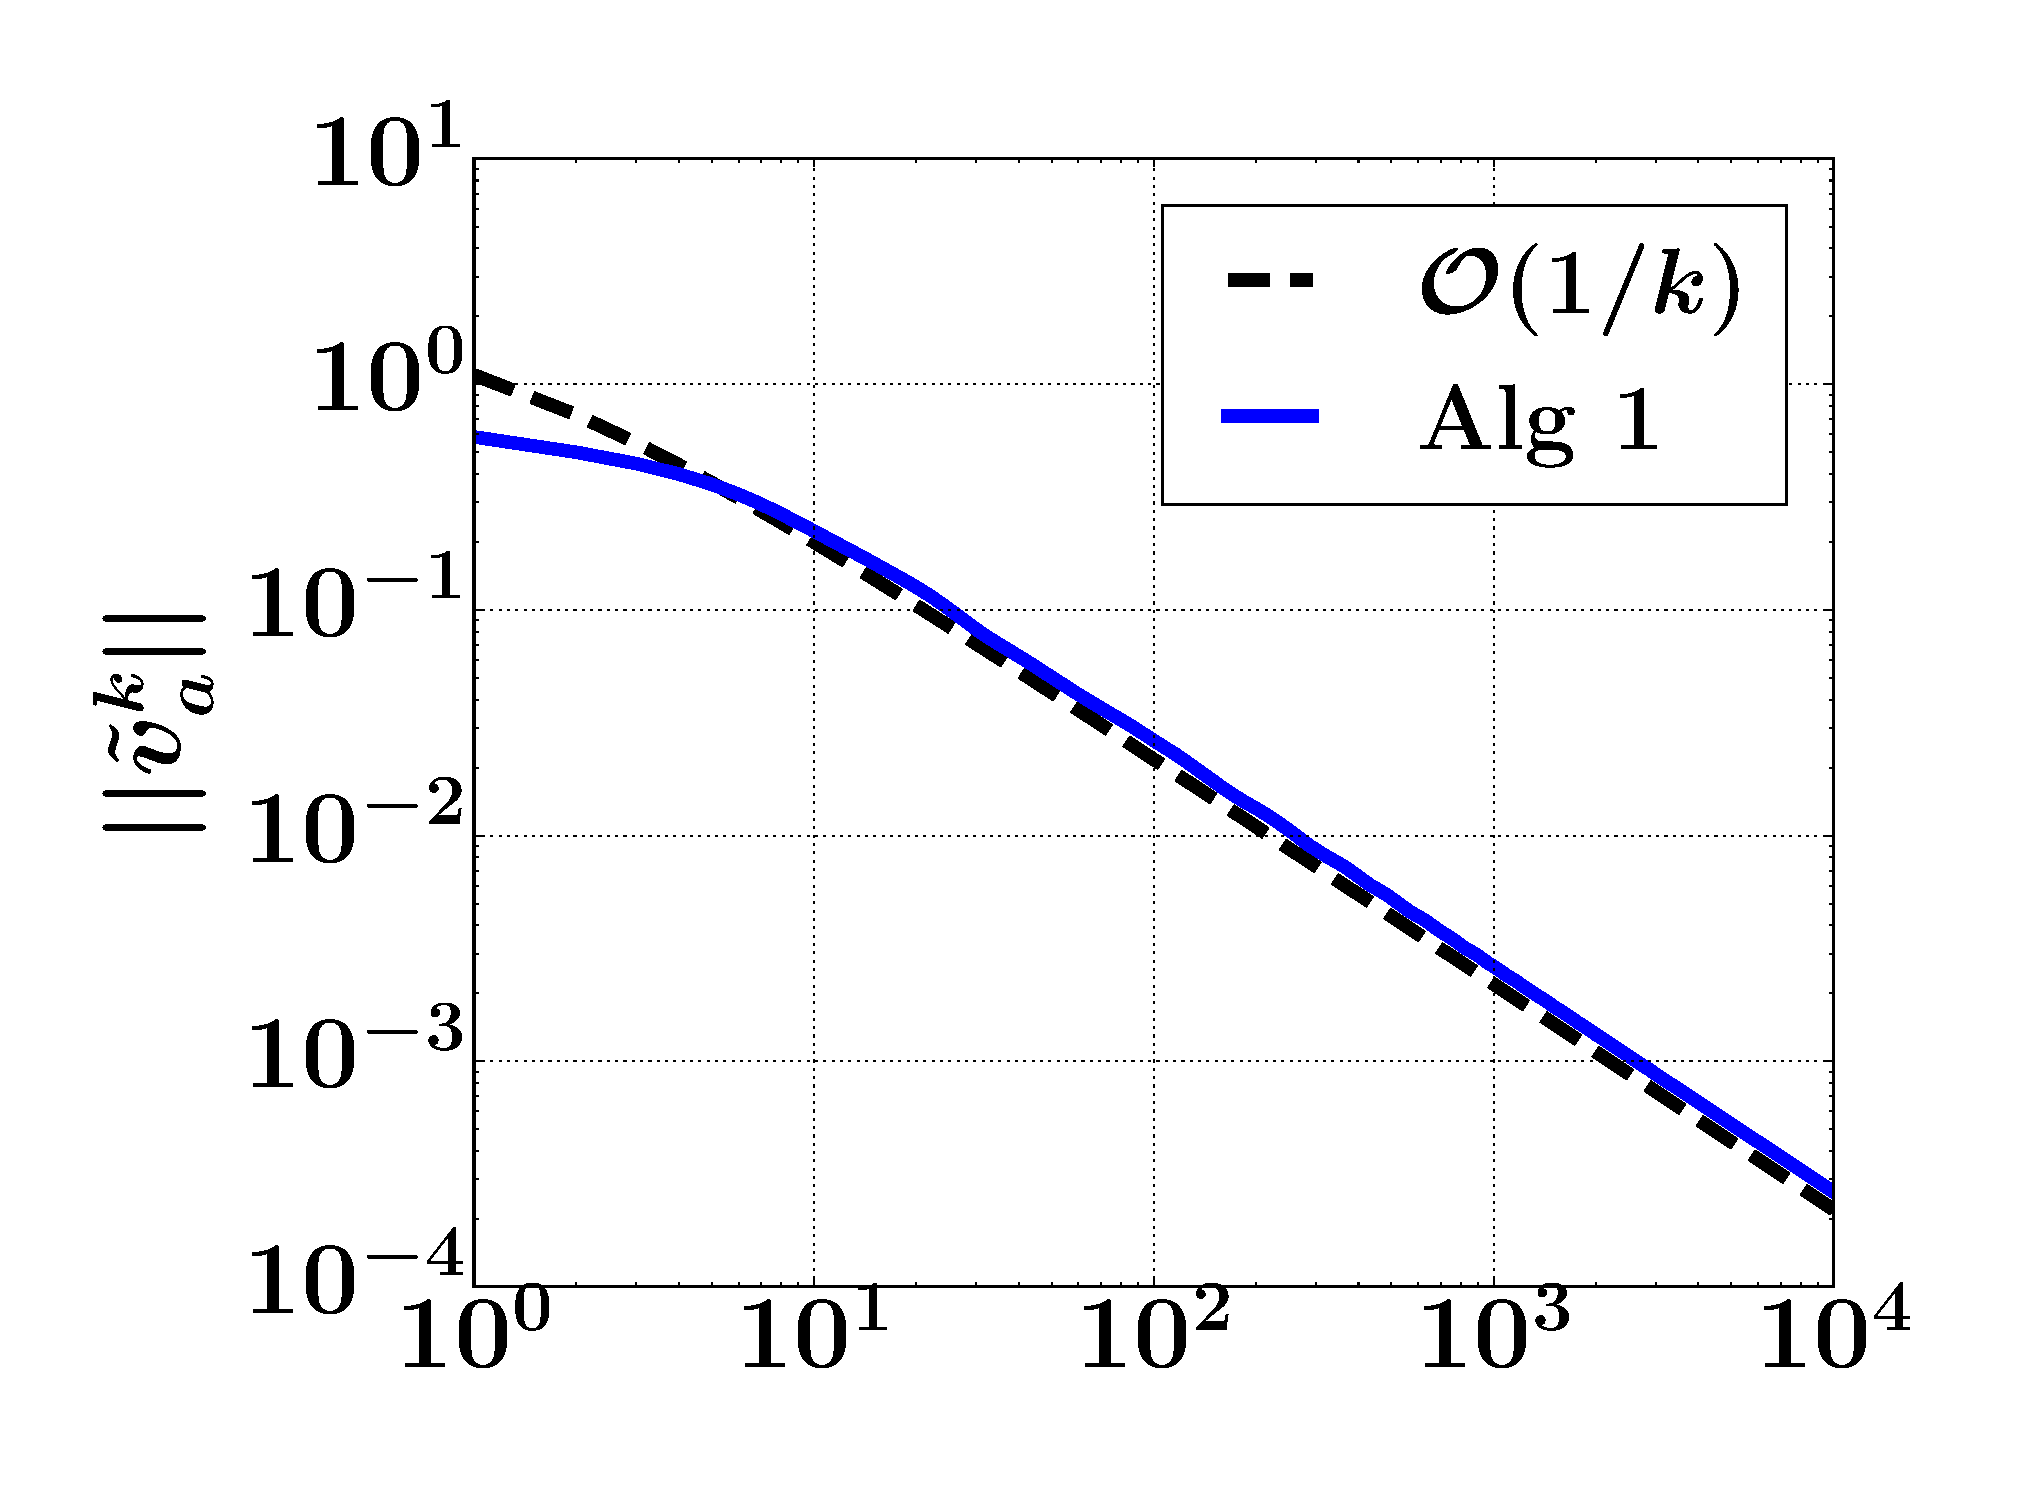
\includegraphics[width=1\linewidth]{simplex_dgap.pdf}
  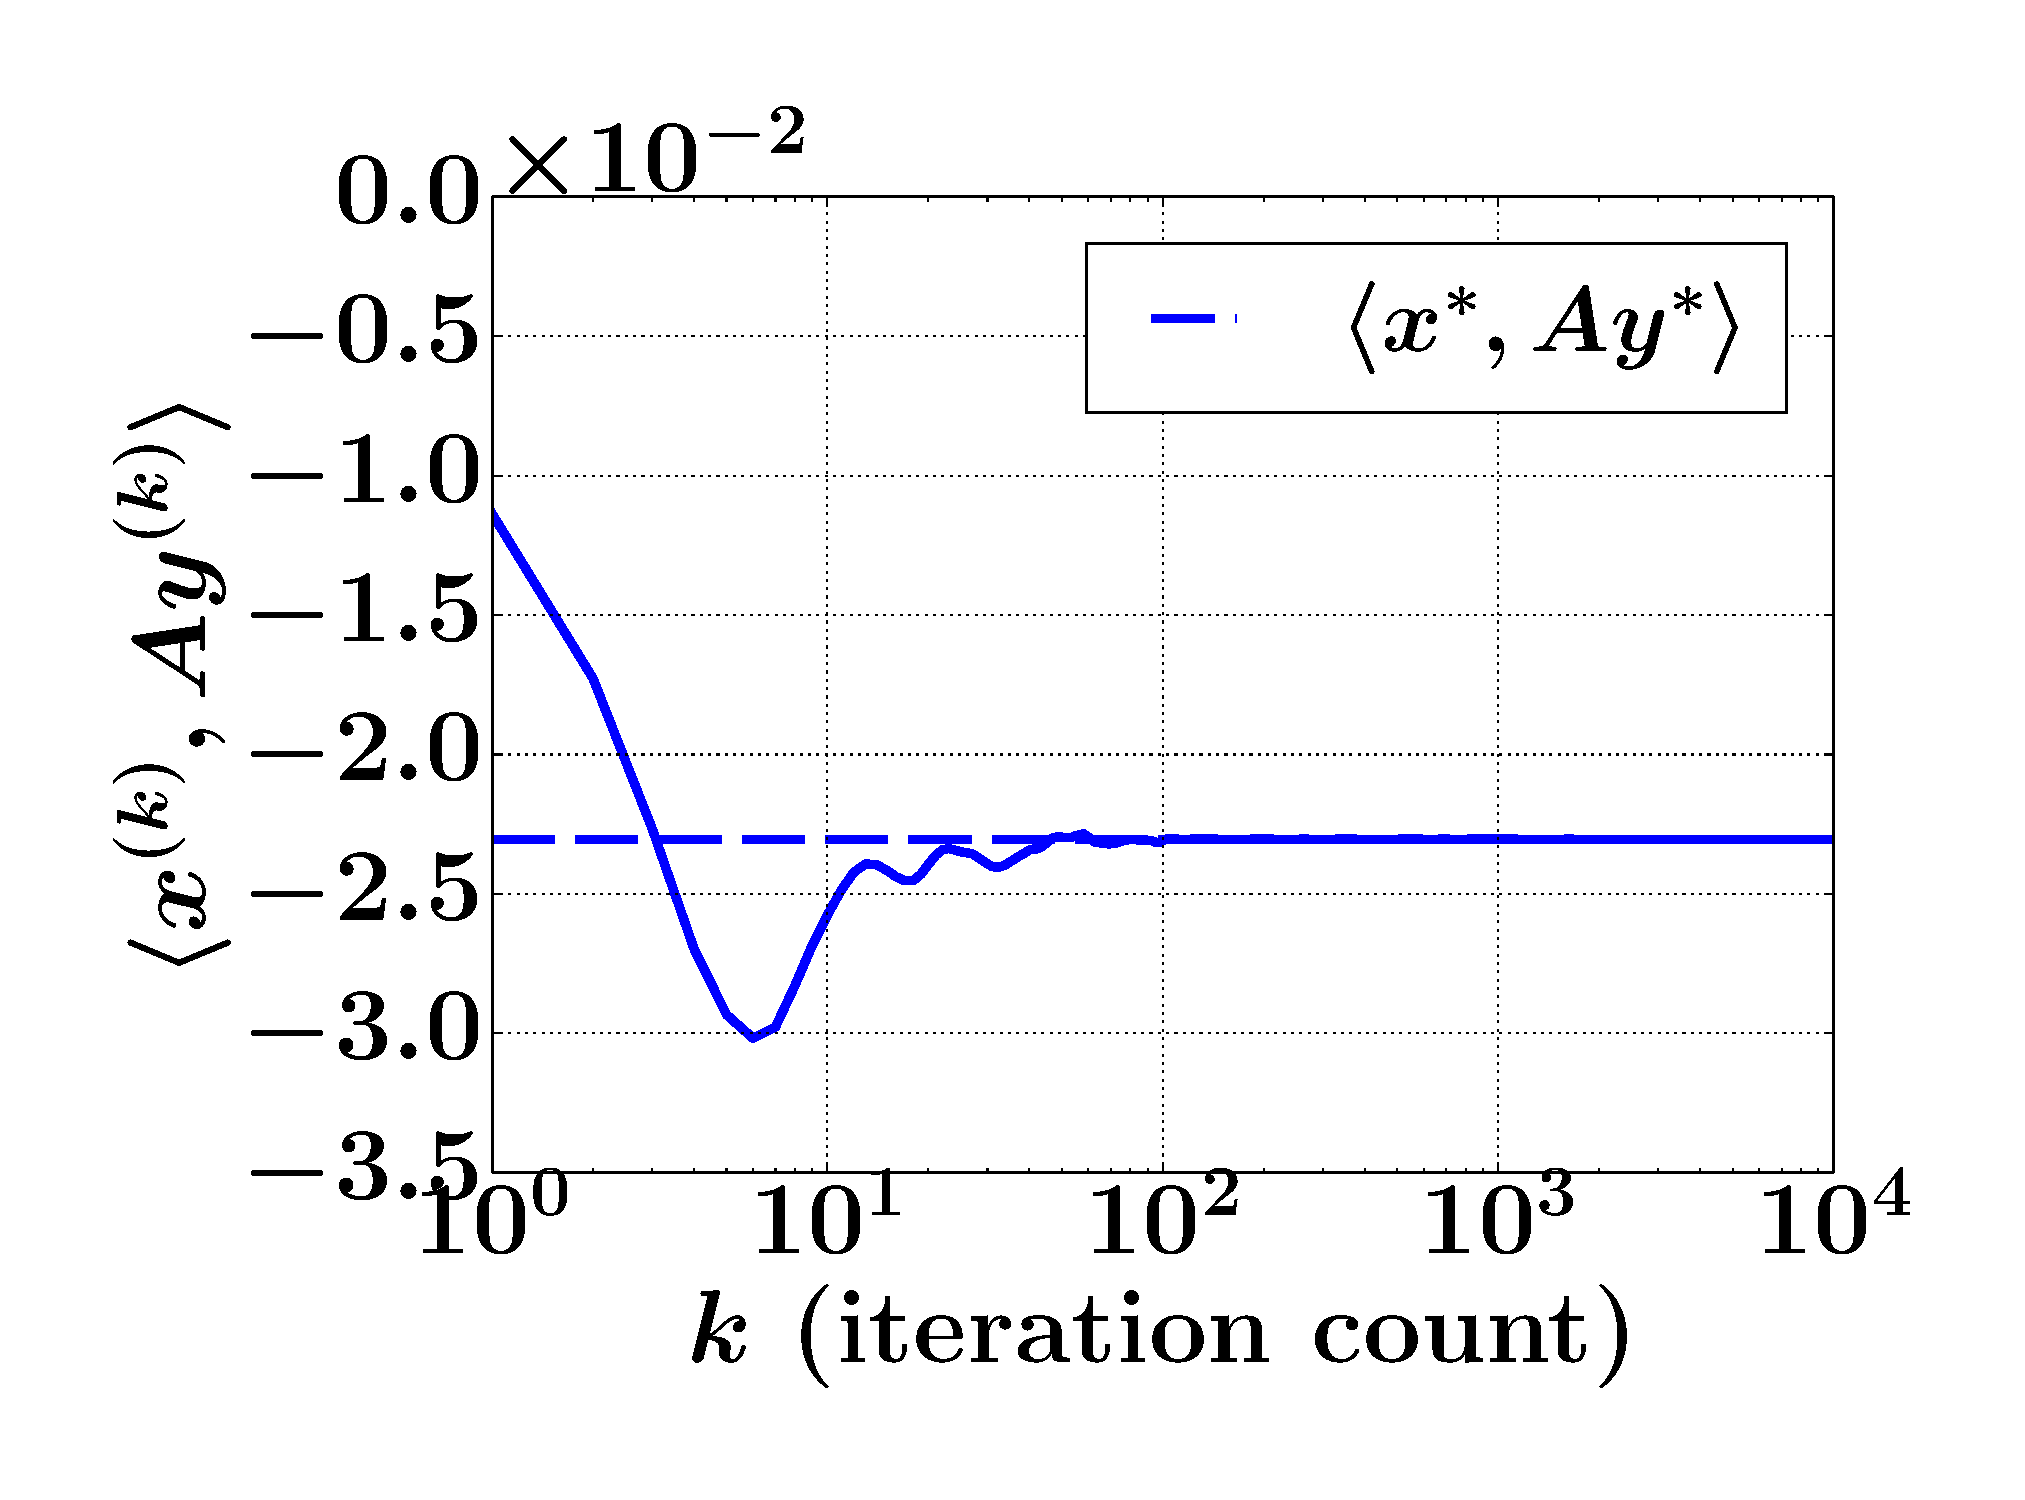
\includegraphics[width=1\linewidth]{simplex_NE.pdf}
  \caption{Convergence curves of Algorithm \ref{Tab:algo_simplified} random $1000 \times 1000$ matrix game (on simplexes)}
  \label{Tab:sim_dgap_curve}
\end{figure}

\subsection{Real-world game: Kuhn 3-card Poker}
The sequence-form representation of this simplified Poker variant was given in subsection \ref{sec:kuhn_sf}. The pair $(x^*, y^*)$ of realization plans given by
$x^* = [1, 0.759, 0.759, 0, 0.241, 1, 0.425, 0.575, 0, 0.275, 0, 0.275, 0.725]^T$ and
$y^* = [1, 1, 0, 0.667, 0.333, 0.667, 0.333, 1, 0, 0, 1, 0, 1]^T$ is a Nash $10^{-4}$-equlibrium.
computed by Algorithm  \ref{Tab:algo_simplified}. The convergence curve is shown in Fig \ref{Tab:dgap_curve}. One easy checks that this equilibrium is feasible. Indeed,  $E_1x^* - e_1 = [4.76 \times 10^{-5}, -1.91 \times 10^{-5}, 5.67 \times 10^{-5}, 8.23 \times 10^{-6}, 2.90 \times 10^{-5}, -8.62 \times 10^{-7}, -1.96 \times 10^{-5}]^T$ and $E_2y^* - e_2 = [-7.04 \times 10^{-7}, 2.27 \times 10^{-6}, -3.29 \times 10^{-6}, -1.50 \times 10^{-6}, 2.92 \times 10^{-6}, -4.97 \times 10^{-7}, -5.85 \times 10^{-7}]^T$. Finally, $x^*TAy^* = -0.055593685705289997$, which agrees to 4 d.p with the value of $-1 / 18$ computed analytically by H. W. Kuhn in his 1950 paper \cite{kuhn}.

The evolution of the dual gap and the expected value of the game across iterations is shown in Figure \ref{Tab:dgap_curve}. These figures validates the theoritically established $\mathcal{O}(1/\epsilon)$ convergence rate of the Algorithm.

\begin{remark}
The results of the experiments presented here are not benchmarks comparing our algorithm to other algorithms, though it would be nice to do such benchmarks in a future work.
\end{remark}

\begin{figure}
  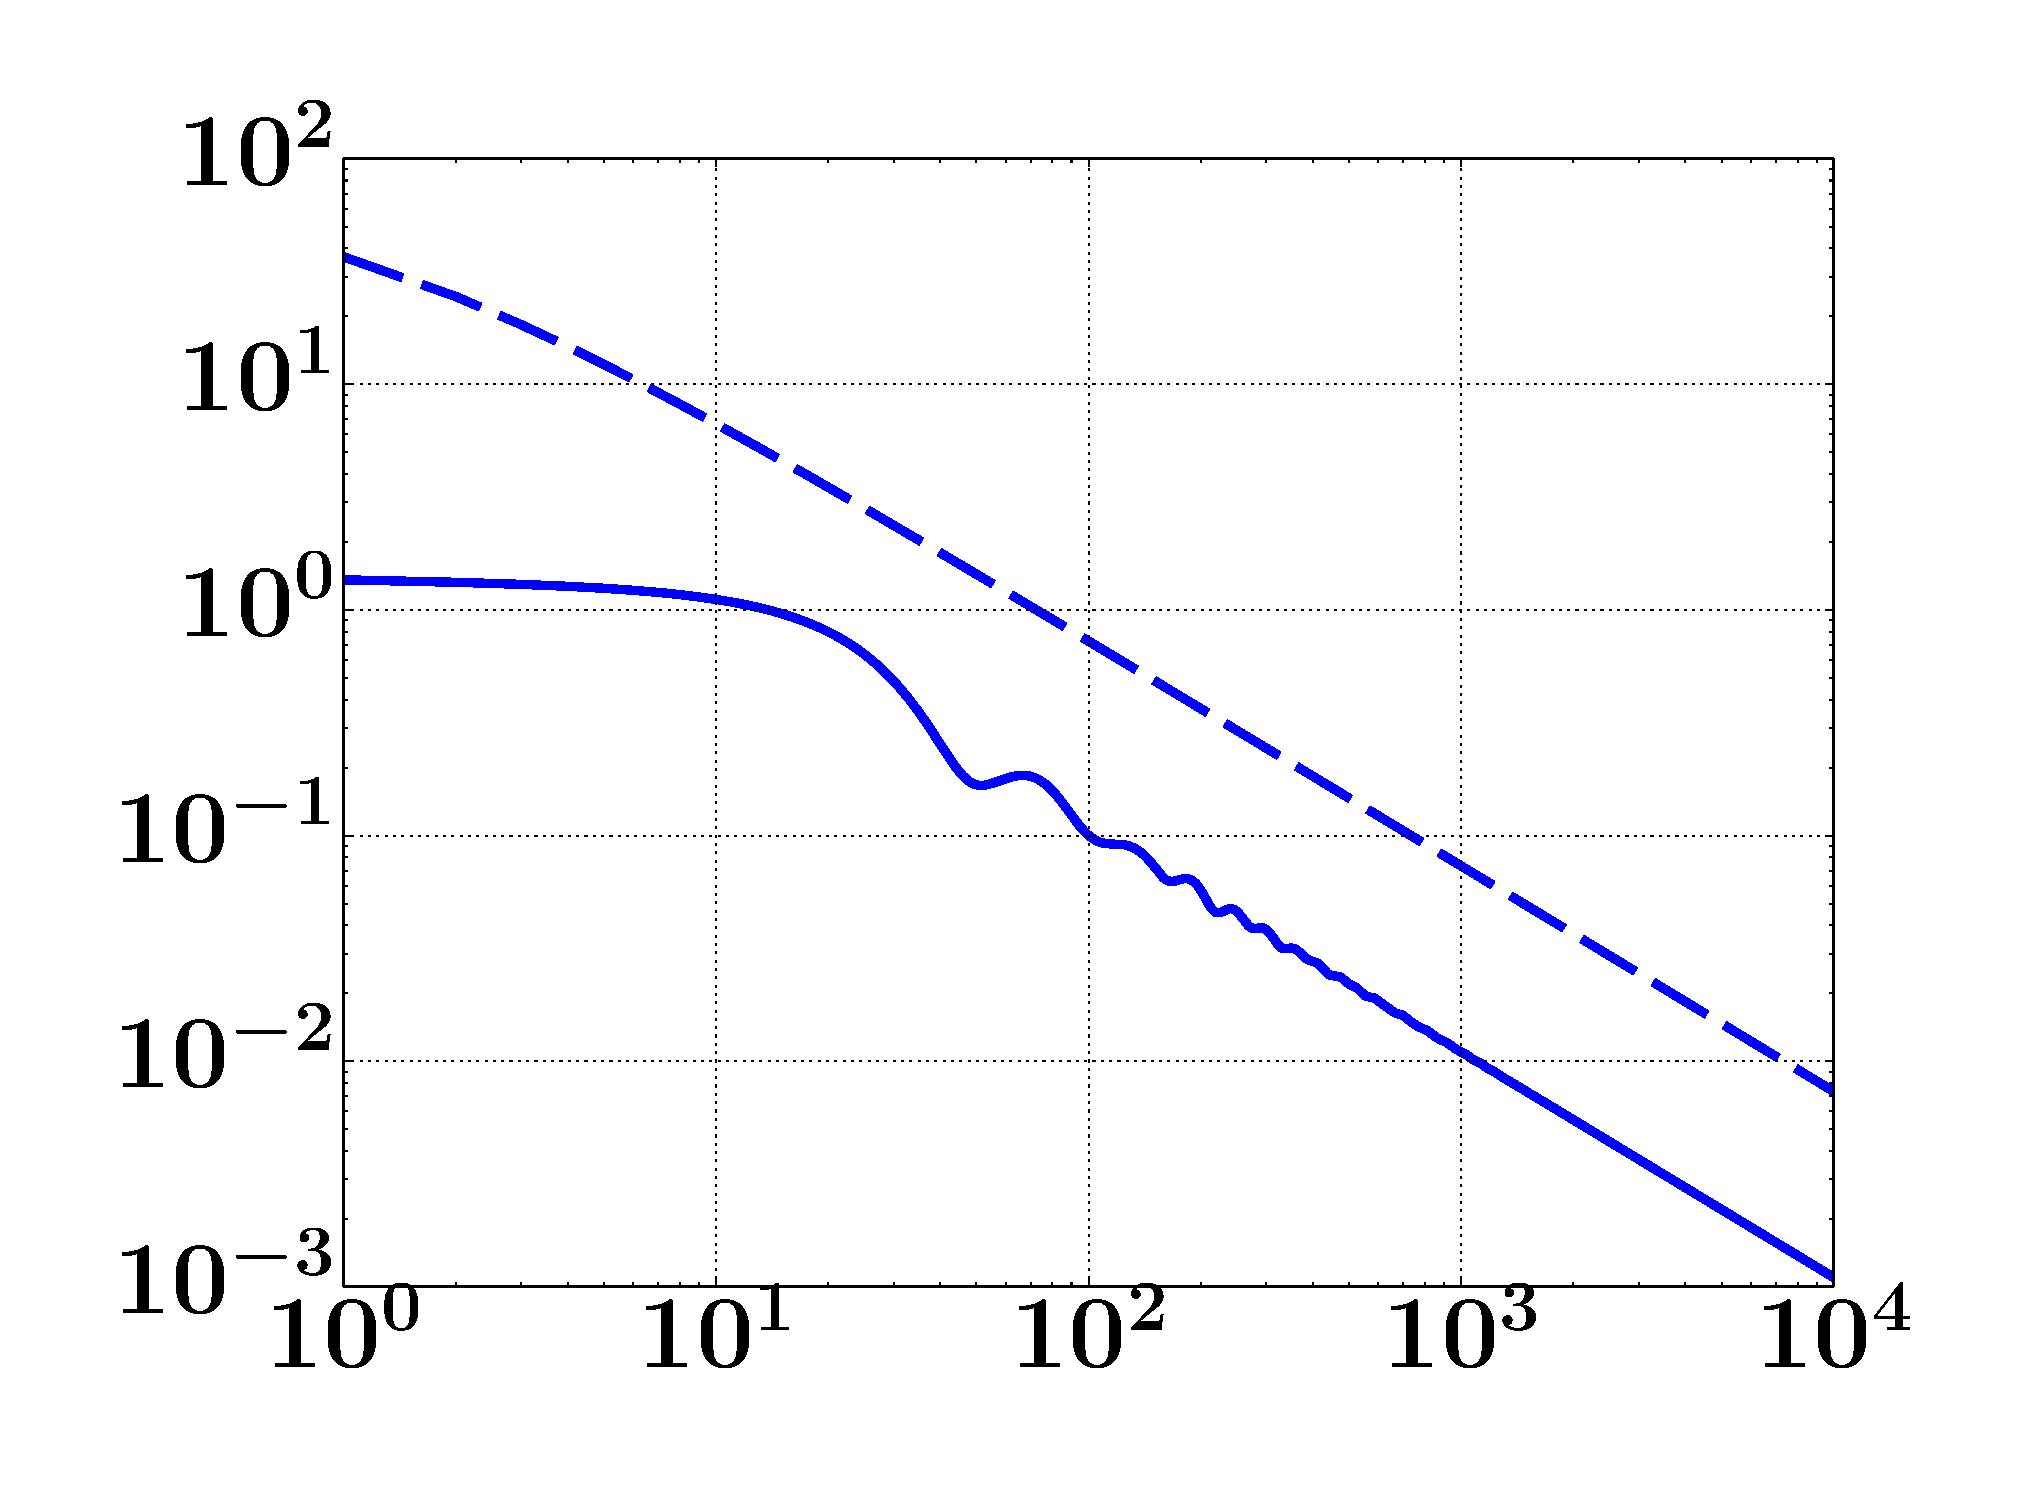
\includegraphics[width=1\linewidth]{Kuhn3112_dgap.pdf}
  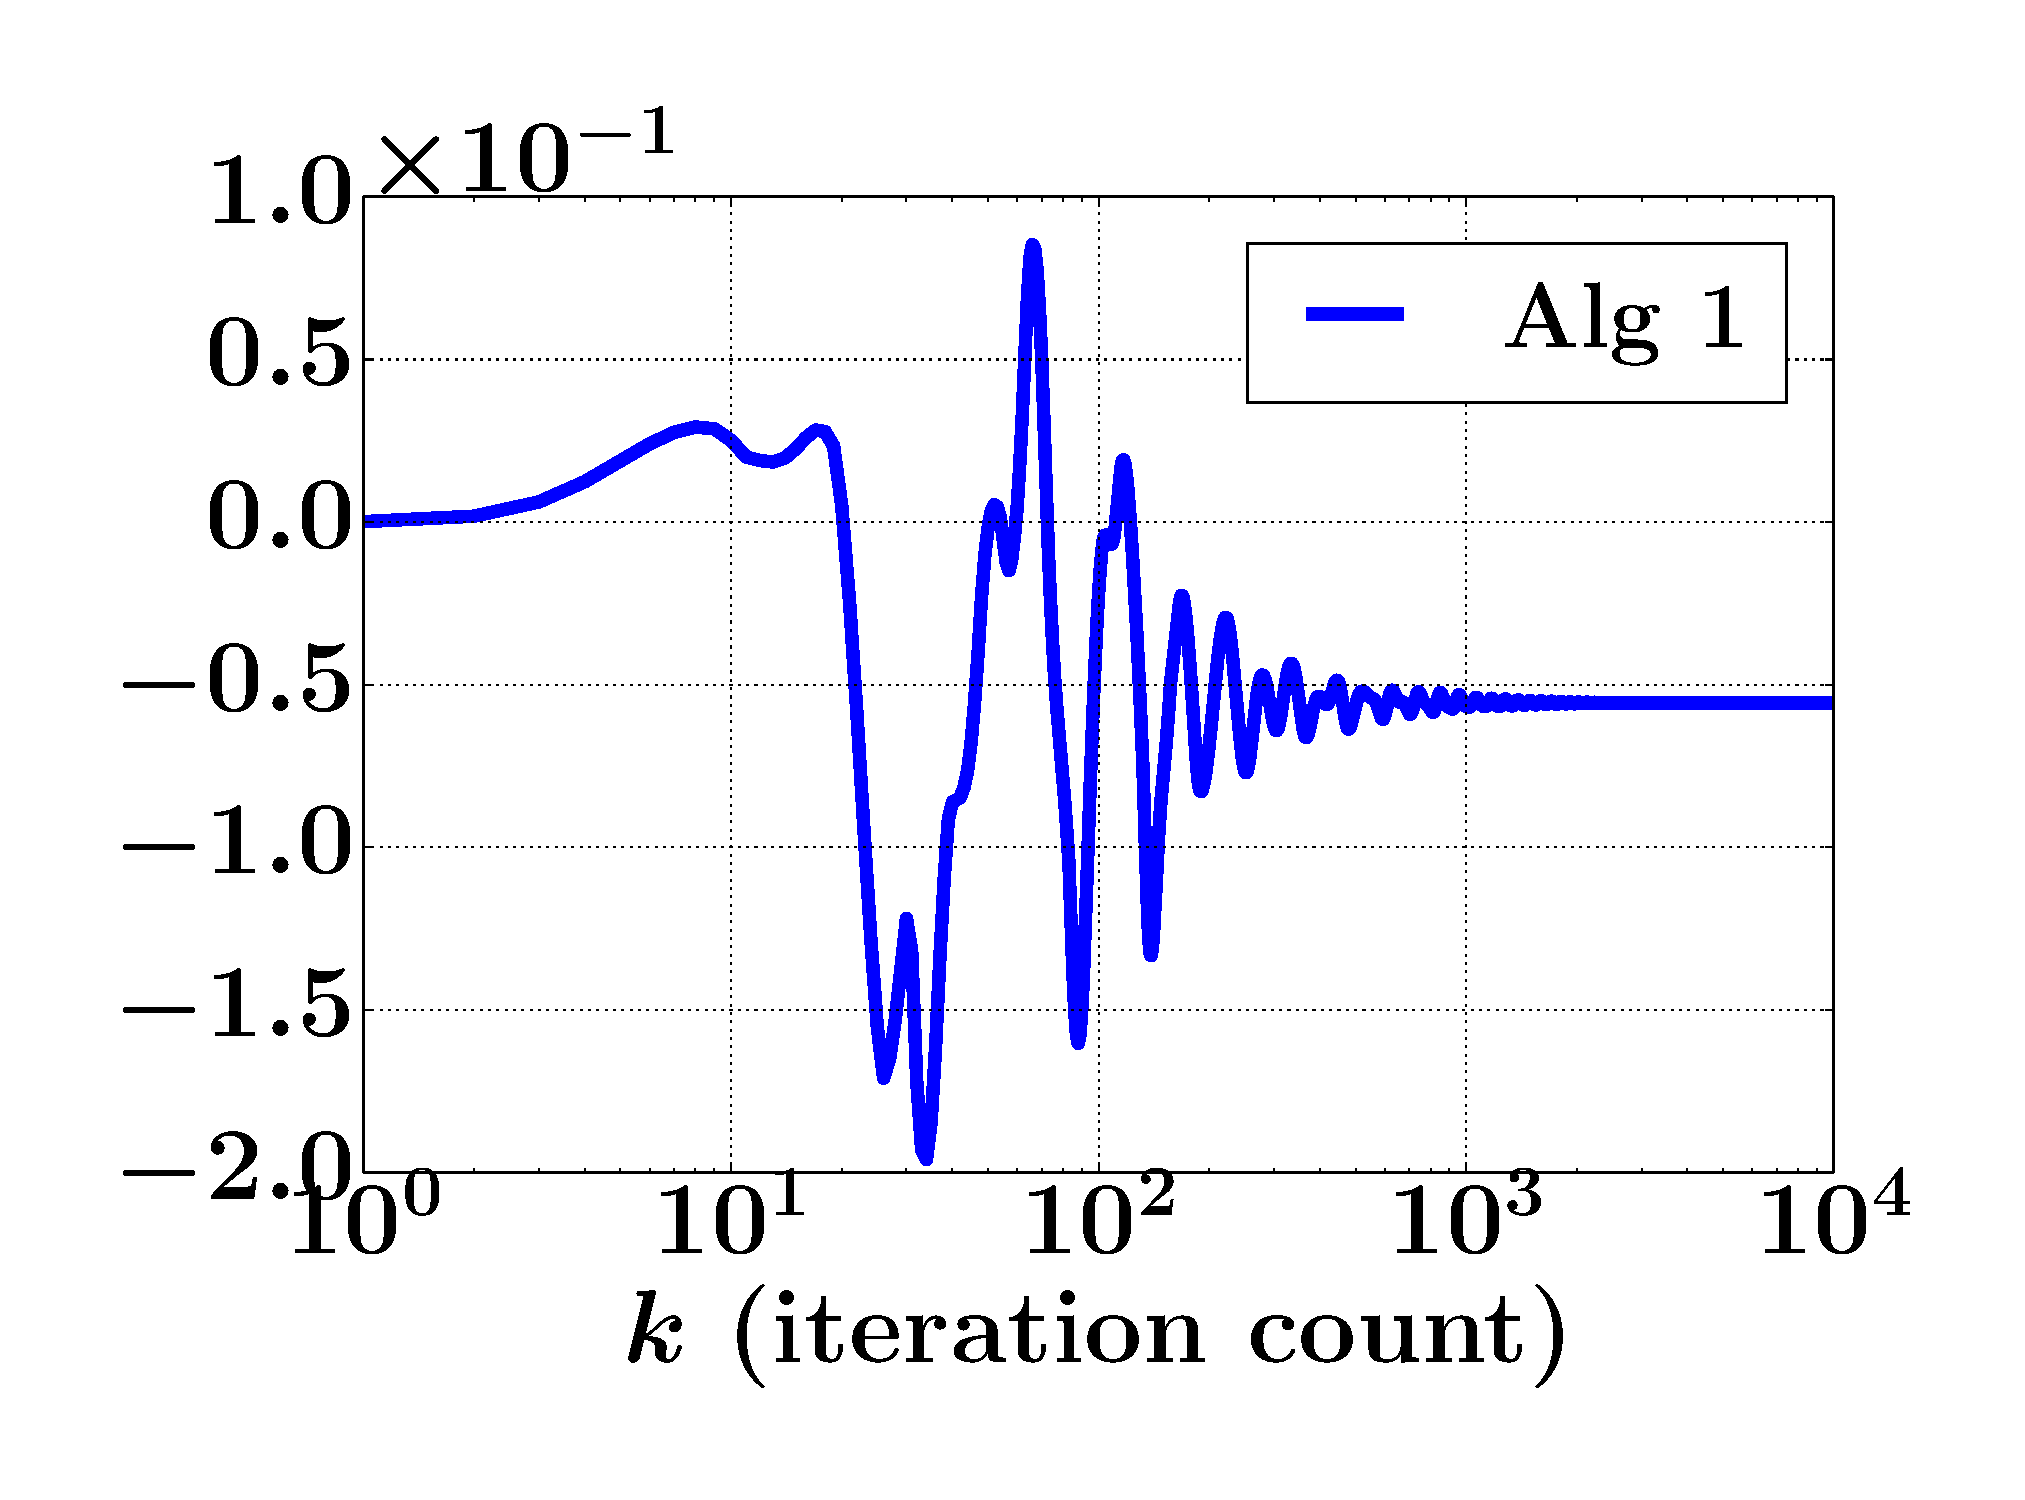
\includegraphics[width=1\linewidth]{Kuhn3112_NE.pdf}
  \caption{Convergence curves of Algorithm \ref{Tab:algo_simplified} on Kuhn 3-card Poker}
  \label{Tab:dgap_curve}
\end{figure}

%% \section{Extending to games with more general strategy profiles}
%% \label{sec:algo_gen}
%% Notice tha in \eqref{eq:poly}, the strategy profile of player $k$ can be factored as
%% \begin{equation}
%%   Q_k := \{z \in \mathbb{R}^{n_k}_+| E_kz = e_k\text\}
%% \end{equation}

%% The framework presented sofar only demanded we be able to efficiently compute euclidean projections onto the nonnegative orthant $\mathbb{R}^{n_k}_+$, namely nonnegative clipping. This opens perspectives to envisage general two-person zero sum games for which the players' strategy profiles are of the form
%% \begin{equation}
%%   Q_k := \{z \in C_k| E_kz = e_k\text\}
%%   \label{eq:q_gen}
%% \end{equation}
%% where the $C_k$ are arbitrary convex sets for which the euclidean projections $\Pi_{C_k}$ can be effectively computed.
%% % \subsection{Example: Computing best response strategies}

%% As a motivating example, suppose Alice knows a priori that Bob is playing a given realization plan $y_0 \in Q_2$ (for example, take $y_0 = [1, 0, ..., 0]^T \in \mathbb{R}^{n_2}$). Alice seeks a \textit{best response strategy}, namely a strategy $x^* \in Q_1$ such that
%% \begin{equation}
%%   x^TAy_0 \le {x^*}^TAy_0,\text{ } \forall x \in Q_1
%% \end{equation}

%% One observes that this problem is an instance of problem \eqref{eq:primal_pb} with
%% $Q_2 = \{y_0\} = \{z \in C_2| E_2z = e_2\text\}$ and $C_2 = \{y_0\}$. Of course the euclidean projection on $C_2$ is simply the constant map $y \mapsto y_0$.

%% As another motivating example, suppose we know the support ...

%% Indeed we have the following generalization of Theorem \ref{thm:pd} for Nash equilibrium problems in which the strategy  profiles have the generic form \eqref{eq:q_gen}.
%% \begin{theorem}
%%   The Nash equilibrium problem \eqref{eq:primal_pb} with strategy profiles given by  equation \eqref{eq:q_gen}, can be re-written in the equivalent unconstrained form
  
%%   \begin{equation}
%%     \underset{y \in \mathbb{R}^{n_2}, v\in \mathbb{R}^{l_1}}{minimize}\text{ }\underset{x \in \mathbb{R}^{n_1}, u \in \mathbb{R}^{l_2}}{maximize}
%%            {\begin{bmatrix}x\\u\end{bmatrix}^TK\begin{bmatrix}y\\v\end{bmatrix} + G_1(y, v) - G_2(x, u)}
%%            \label{eq:unconstrained_gen_pb}
%%   \end{equation}

%%   where $v \in \mathbb{R}^{l_1}$ and $u \in \mathbb{R}^{l_2}$ are auxiliary variables and 
%%   \begin{equation}
%%     \left .
%%     \begin{split}
%%       K :=
%%       \left[
%%         \begin{array}{c|c}
%%           A & -E_1^T \\ \hline
%%           E_2 & 0_{l_2, l_1}
%%         \end{array}
%%         \right] \in \mathbb{R}^{(n_1 + l_2) \times (n_2 + l_1)} \\
%%       %%\begin{bmatrix}A \text{ } E_1^T\\ E_2 \text{ } 0\end{bmatrix} \in \mathbb{R}^{(n_2 + l_1) \times (n_1 + l_2)}\\
%%       G_1: \mathbb{R}^{n_2} \times \mathbb{R}^{l_1} \rightarrow [-\infty, +\infty], (y, v) \mapsto i_{C_2}(y) + e_1^Tv\\
%%       G_2: \mathbb{R}^{n_1} \times \mathbb{R}^{l_2} \rightarrow [-\infty, +\infty], (x, u) \mapsto i_{C_1}(x) + e_2^Tu
%%     \end{split}
%%     \right\}
%%     \label{eq:things}
%%   \end{equation}
  
%%   Moreover, $G_1$ and $G_2$ are \textit{p.c.l.s.c} and their proximal operators are given by
%%   \begin{equation}
%%     \left .
%%     \begin{split}
%%       \text{prox}_{\tau G_1} : \mathbb{R}^{n_2} \times \mathbb{R}^{l_1} &\rightarrow \mathbb{R}^{n_2} \times \mathbb{R}^{l_1}\\
%%       (y, v) &\mapsto (\Pi_{C_2}(y), v - \tau e_1)\\
%%     \end{split}
%%     \right\}
%%   \end{equation}

%%   and
%%   \begin{equation}
%%     \left .
%%     \begin{split}
%%       \text{prox}_{\sigma F}: \mathbb{R}^{n_1} \times \mathbb{R}^{l_2} &\rightarrow \mathbb{R}^{n_1} \times \mathbb{R}^{l_2}\\
%%       (x, u) &\mapsto (\Pi_{C_1}(x), u - \sigma e_2)
%%     \end{split}
%%     \right\}
%%   \end{equation}
%%   \label{thm:pd_gen}
%% \end{theorem}

%% \begin{proof}
%% Totally analogous to the proof of Theorem \ref{thm:pd} with $\mathbb{R}^{n_k}_+$ replaced with $C_k$,
%% $i_{\mathbb{R}^{n_k}_+}$ replaced with $i_{C_k}$, and $\Pi_{\mathbb{R}^{n_k}_+}$ (nonnegative clipping) replaced with $\Pi_{C_k}$.
%% \end{proof}

%% %\subsection{$\mathcal{O}(1/\epsilon)$ primal-dual algorithm for general problems}
%% Analogous to Algorithm \ref{Tab:algo_simplified}, we obtain Algorithm \ref{Tab:algo} for solving the Nash equilibrium problem \ref{eq:primal_pb} with the general strategy profiles $Q_k$ defined in \eqref{eq:q_gen}. Just like Algorithm \ref{Tab:algo_simplified}, Algorithm \ref{Tab:algo} has a $\mathcal{O}(1/\epsilon)$ convergence rate.

%% \begin{algorithm}[G_2yy]
%%   \caption{$\mathcal{O}(1/\epsilon)$ Primal-dual algorithm for solving the Nash equilibrium problem \eqref{eq:primal_pb}, with general strategy profiles as defined in \eqref{eq:q_gen}}
%%   \KwIn{specification of a game $(A, E_1, E_2, e_1, e_2, C_1, C_2)$, where $A \in \mathbb{R}^{n_1 \times n_2}$,
%%       $E_1 \in \mathbb{R}^{l_1 \times n_1}$, $E_2 \in \mathbb{R}^{l_2 \times n_2}$, $e_1 \in \mathbb{R}^{l_1}$, $e_2 \in \mathbb{R}^{l_2}$, each $C_k$ is a convex subset of $\mathbb{R}^{n_k}$, as in the definition of the strategy profiles $Q_k$ in equation \eqref{eq:q_gen}}
%%   \KwOut{Nash $\epsilon-$equilibrium pair $x^{(k)}$, $y^{(k)}$}
%%   \textbf{Precompute}: $\|K\|^2$, where $K$ is constructed as in equations \eqref{eq:unconstrained_pb}. $\|K\|^2$ can be computed via a \textit{power iteration} on $K^TK$, for example.\\
%%   \textbf{Initialize}:
%%   $x^{(0)} \in \mathbb{R}^{n_1}$; $v \in \mathbb{R}^{l_1}$; $\tilde{y^{(0)}}, y^{(0)} \in \mathbb{R}^{n_2}$; $u^{(0)} \in \mathbb{R}^{l_2}$; 
%%   $\tau, \sigma > 0 \text{ s.t. }\tau\sigma \|K\|^2 < 1$ (for example take $\tau = \sigma = .99/\|K\|$); $k = 0$.\\
%%   \While{
%% %$\dfrac{\| x^{(k+1)} - x^{(k)}\|^2 + \|v^{(k+1)}- v^{(k)}\|^2}{\sigma} + \dfrac{\|y^{(k+1)}- y^{(k)}\|^2 + \|u^{(k+1)}- u^{(k)}\|^2}{\tau} < \epsilon$
%% $|p^Te_1^{(k)} - q^Te_2^{(k)}| \geq \epsilon$}{
%%     \begin{eqnarray*}
%%       x^{(k+1)} &\leftarrow& \Pi_{C_1}\left(x^{(k)} + \tau \left(A\tilde{y}^{(k)} - E_1^T\tilde{v}^{(k)}\right)\right)\\
%%       u^{(k+1)} &\leftarrow& u^{(k)} + \tau \left(E_2\tilde{y}^{(k)} - e_2\right)\\
%%       y^{(k+1)} &\leftarrow& \Pi_{C_2}\left(y^{(k)} - \sigma \left(A^Tx^{(k + 1)} + E_2^Tu^{(k + 1)}\right)\right)\\
%%       v^{(k+1)} &\leftarrow& v^{(k)} - \sigma \left(e_1 - E_1x^{(k+1)}\right)\\
%%       \tilde{y}^{(k+1)} &\leftarrow& 2y^{(k+1)} - y^{(k)}\\
%%       \tilde{u}^{(k+1)} &\leftarrow& 2u^{(k+1)} - u^{(k)}\\
%%       k &\leftarrow& k + 1
%%     \end{eqnarray*}
%%   }
%%   \label{Tab:algo}
%% \end{algorithm}

\section{Conclusion}
For the first time, we have applied a primal-dual algorithm to the problem of computing Nash equilibria for two-person zero-sum sequential games with imcomplete information (like Texas Hold'em, etc.). Our algorithm is simple to implement, with a very low constant cost per iteration, and enjoys a rigorous convergence theory with a proven $\mathcal{O}(1/\epsilon)$ convergence in terms of basic operations (matvec products, clipping, etc.), to a Nash $\epsilon$-equilibrium of the game...

\medskip \noindent
\textbf{About the author:} I'm a first-year PhD student in Computer Science at Universit\'e de Parix XI. My thesis focuses on novel techniques for optimization on Lie groups (of diffeomorphisms), and other structured manifolds, the aim being to obtain better algorithms for nonlinear registration of fMRI brain images and enhance the charting of human functional connectomes.

\textbf{Acknowledgments:} ...
\small
\bibliographystyle{agsm}
% \bibliographystyle{abbrvnat}
\bibliography{bib}

\end{document}
